%------------------------------------------
%   1.	Periodic (Born–von Karman) Boundary Conditions
%------------------------------------------
\section{Periodic (Born–von Karman) Boundary Conditions}
Xét bài toán tính số electron có thể tồn tại trong một sợi dây đồng với chiều dài $L$ ở một mức năng lượng nhất định. 
Bài toán này có thể giải theo nhiều cách nhưng trong Solid-state có một cách rất hay là dùng điều kiện biên tuần hoàn, tức là ta biến sợi dây này thành 1 vòng tròn, 
khi đó electron này sẽ chỉ chạy quanh vòng tròn này. Hàm sóng cho bất kỳ electron trong vòng này là 
    \eq{1.1}{e^{ikr}.}
Hàm sóng này có các giá trị như nhau tại vị trí $r$ và $r +L$, tức là ta đi hết 1 vòng tròn, trong đó giá trị của $k$ là
    \eq{1.2}{k = \frac{2\pi n}{L}.}
Với chiều dài $L$ đủ lớn thì ta được phép thay tổng bằng một tích phân sau\footnote{Để biết chiều dài đủ lớn thì bạn so sánh chiều dài với kích thước của electron.}
    \eq{1.3}{\sum_k \rightarrow \frac{L}{2\pi}\int_{-\infty}^{\infty}dk.}
Để hiểu phép ánh xạ này một cách đơn giản là giữa các điểm trong không gian $k$ sẽ có khoảng cách là $L/2\pi$ (điều này quyết định mật độ trạng thái trong không gian $k$)
nên ta có thể thay thế tổng rời rạc bằng tích phân liên tục nhân vơi khoảng cách giữa các điểm đó.  
    \begin{more}
        \textit{Vu vơ thêm:} Tại sao hệ số $L/2\pi$ lại là mật độ trạng thái. Ta có
        \eqs{\Delta k = \frac{2\pi}{L}.}
        Khi xét mật độ trạng thái tức là
        \eqs{\frac{1}{\Delta k} = \frac{L}{2\pi}.}
        Tổng rời rạc theo $k$ ở trên tức là ta đang cộng từng điểm $k$ có trong không gian và mỗi điểm cách nhau một khoảng $\Delta k$. Khi đó
        \eqs{\sum_k \approx \sum_k \Delta k \times \frac{1}{\Delta k} \rightarrow \frac{L}{2\pi}\int_{-\infty}^{\infty}dk.}
    \end{more}
Tất cả những lập luận trên đều là đang xét trong bài toán một chiều, khi mở rộng ra bài toán 3 chiều thì ta thu được
    \eq{1.4}{\sum_{\mathbf{k}} \rightarrow \left(\frac{L}{2\pi}\right)^3 \int_{-\infty}^{\infty}d\mathbf{k}.}
%------------------------------------------
%   2.	Evolution of Heat Capacity Models
%------------------------------------------
\section{Evolution of Heat Capacity Models}
\subsection{The law of Dulong - Petit}
Năm 1819, theo định luật Dulong - Petit\footnote{Định luật này được đề xuất bởi 2 nhà vật lý người pháp là Pierre Louis Dulong (1785 - 1838) và Alexis Thérèse Petit (1791 - 1820). Cả hai đều không được nhớ đến nhiều ngoài định luật này.} thì nhiệt dung được cho bởi
    \eq{1.5}{C = 3k_B \quad \text{trên mỗi nguyên tử}}
Trong đó $k_B$ là hằng số Boltzmann. Trong xuyên suốt ta sẽ luôn quan tâm đến nhiệt dung $C$ trên mỗi nguyên tử của bất kỳ vật liệu nào,
ở đây ta sẽ không phân biệt giữa nhiệt dung đẳng áp $C_p$ và nhiệt dung đẳng tích $C_v$ bởi lẽ giá trị của chúng không chênh lệch nhau quá nhiều.
Định luật này mặc dù rất gần với thực tế nhưng có một vài trường hợp thì định luật này không phù hợp. 
\tab{Nhiệt dung của một vài chất rắn ở nhiệt độ và áp suất phòng}{bang1}{
    \begin{tabular}{lc} 
        \toprule 
        Vật liệu & $C/R$ \\ 
        \midrule 
        Nhôm (Al) & 2.91 \\
        Chì (Pb) & 3.03 \\
        Đồng (Cu) & 2.94 \\
        Vàng (Au) & 3.05 \\
        Bạc (Ag) & 2.99 \\
        Kim cương (C) & 0.735\\
        \bottomrule 
    \end{tabular}
}\\
Như đã thấy trong bảng~\ref{tab:bang1} thì ngoại trừ kim cương thì các vật liệu khác gần như đúng với định luật $C/R=3$ ở nhiệt độ cao. Tuy nhiên, khi nhiệt độ giảm, kết quả thực nghiệm cho thấy nhiệt dung giảm mạnh và tiến về 0, mâu thuẫn với dự đoán cổ điển.
Trong mô tả cổ điển, khi mà mỗi nguyên tử trong một mạng tinh thể được xem như dao động quanh vị trí cân bằng trong một thế điều hòa do tương tác với các nguyên tử lân cận. Kết hợp với định lý phân bố đều năng lượng, mô hình này dẫn đến kết quả $C=3k_b$ trên mỗi nguyên tử, phù hợp với định luật Dulong - Petit. Tuy nhiên, vẫn thất bại ở nhiệt độ thấp.
Sau đó vào năm 1907, dựa trên mô hình dao động điều hòa cổ điển, Einstein đã đề xuất một mô hình lượng tử cho chất rắn, trong đó giả định mọi nguyên tử đều nằm trong một giếng thế điều hòa giống hệt nhau và có tần số dao động là $\omega$, tần số này được gọi là tần số "Einstein".
\subsection{Einstein's Calculation}
Năng lượng của dao động tử điều hòa trong một chiều được cho bởi
    \eq{1.6}{E_n = \left(n + \frac{1}{2}\right)\hbar \omega, \quad n = 0, 1, 2, \ldots}
Trong đó $\hbar$ là hằng số Planck rút gọn và $\omega$ là tần số dao động của nguyên tử trong mạng tinh thể (hoặc tần số "Einstein").\\
Trong vật lý thống kê, ta có tổng thống kê chính tắc lượng tử được cho bởi
    \eq{1.7}{\mathcal{Z} = \sum_{n\geq 0} e^{-E_n/k_B T}=\frac{1}{2\sinh(\beta\hbar\omega/2)}.} 
    \begin{more}
        \textit{Làm toán tí}: Ta có 
        \eqs{
            \begin{aligned}
                \mathcal{Z} &= \sum_{n\geq 0} e^{-E_n/k_B T}\\
                &= \sum_{n\geq 0} e^{-\beta\hbar\omega(n+1/2)}\\
                &= e^{-\beta\hbar\omega/2} \sum_{n\geq 0} e^{-\beta\hbar\omega n}\\
                &= e^{-\beta\hbar\omega/2} \frac{1}{1 - e^{-\beta\hbar\omega}}\\
                &= \frac{1}{2\sinh(\beta\hbar\omega/2)}. 
            \end{aligned}
        }
        Ở đây ta đặt $\beta = 1/k_B T$.
    \end{more}
Khi đó ta có giá trị kỳ vọng của năng lượng là 
    \eq{1.8}{\langle E \rangle = -\frac{1}{\mathcal{Z}} \frac{\partial \mathcal{Z}}{\partial \beta} = \hbar\omega\left(n_B(\beta\hbar\omega) + \frac{1}{2}\right).}
    Mode dao động có tần số $\omega$ được mô tả như một mode boson có số chiếm trung bình là $n_B(\beta\hbar\omega)$, tương ứng với số lượng kích thích lượng tử trung bình trong mode đó.
    \begin{more}
        \textit{Làm toán tí}: Ta có 2 cách để khai triển biểu thức này như sau\\
            \begin{minipage}[t]{0.4\textwidth}
                \vspace{0pt}
                \textbf{Cách 1}
                \eqs{
                \begin{aligned}
                    \langle E \rangle &= -\frac{1}{\mathcal{Z}} \frac{\partial \mathcal{Z}}{\partial \beta}\\
                    &= - \frac{\partial}{\partial \beta} \ln{\mathcal{Z}}\\
                    &= -\frac{\partial}{\partial \beta} \left(-\ln(2\sinh(\beta\hbar\omega/2))\right)\\
                    &= \frac{\hbar\omega}{2} \coth(\beta\hbar\omega/2)\\
                    &= \hbar\omega\left(\frac{1}{e^{\beta\hbar\omega} - 1} + \frac{1}{2}\right)\\
                    &= \hbar\omega\left(n_B(\beta\hbar\omega) + \frac{1}{2}\right).
                \end{aligned}
                }
            \end{minipage}
            \hfill
            \begin{minipage}[t]{0.5\textwidth}
            \vspace{0pt}
            \textbf{Cách 2}
                \eqs{
                \begin{aligned}
                    \langle E \rangle &= -\frac{1}{\mathcal{Z}} \frac{\partial \mathcal{Z}}{\partial \beta}\\
                    &= -2\sinh(\beta\hbar\omega/2) \frac{\partial}{\partial \beta} \left(\frac{1}{2\sinh(\beta\hbar\omega/2)}\right)\\
                    &= -2\sinh(\beta\hbar\omega/2) \left(-\frac{\hbar\omega}{2}\right)\frac{\cosh(\beta\hbar\omega/2)}{\sinh^2(\beta\hbar\omega/2)}\\
                    &= \frac{\hbar\omega}{2} \frac{\cosh(\beta\hbar\omega/2)}{\sinh(\beta\hbar\omega/2)}\\
                    &= \frac{1}{2}\hbar\omega \frac{e^x + e^{-x}}{e^x - e^{-x}} \quad (x = \beta\hbar\omega/2)\\
                    &= \frac{1}{2}\hbar\omega\frac{e^{2x} + 1}{e^{2x} - 1}\\
                    &= \frac{1}{2}\hbar\omega\frac{(e^{2x} - 1) + 2}{e^{2x} - 1}\\
                    &= \frac{1}{2}\hbar\omega\left(1 + \frac{2}{e^{2x} - 1}\right)\\
                    &= \hbar\omega\left(\frac{1}{e^{\beta\hbar\omega} - 1} + \frac{1}{2}\right)\\
                    &= \hbar\omega\left(n_B(\beta\hbar\omega) + \frac{1}{2}\right).
                \end{aligned}
                }
            \end{minipage}\\
        Ở đây ta sử dụng hàm phân bố Bose-Einstein là 
        \eqs{n_B(x) = \frac{1}{e^{x} - 1}.}
    \end{more}
Khi đó nhiệt dung cho một dao động tử đơn giản là
    \eq{1.9}{C = \frac{\partial \langle E \rangle}{\partial T} = k_B \left(\beta\hbar\omega\right)^2 \frac{e^{\beta\hbar\omega}}{\left(e^{\beta\hbar\omega} - 1\right)^2}.}
Mở rộng ra 3 chiều thì ta có
    \eq{1.10}{\langle E_{3D}\rangle = 3\langle E_{1D}\rangle \Rightarrow C = 3k_B \left(\beta\hbar\omega\right)^2 \frac{e^{\beta\hbar\omega}}{\left(e^{\beta\hbar\omega} - 1\right)^2}.}
        Nhưng mà khi so sánh với kết quả thực nghiệm thì việc sử dụng tần số ``Einstein''
        để tìm ra phương trình lý thuyết vẫn còn chưa chính xác.
        Điều này là do trong giới hạn nhiệt độ thấp, hầu hết các vật đều có nhiệt dung
        tỉ lệ với $T^3$ nhưng công thức của Einstein lại tuân theo $e^T$,
        nên dẫn đến việc không khớp với các điểm thực nghiệm (xem Hình~\ref{fig:1.1}). \\
\fig{figure/chap1/1.png}{0.5}{So sánh nhiệt dung tính theo mô hình Einstein với kết quả thực nghiệm.}{1.1}
        Một điều dẫn đến kết quả của Einstein sai lệch nhiều
        là do việc ông giả thiết rằng $N$ nguyên tử trong chất rắn dao động độc lập với nhau và đều có cùng tần số $\omega$ nên mô hình này
        đã bỏ qua các tương tác giữa chúng. Khi đó ta sẽ đi tới việc tính toán của Debye có độ chính xác tốt hơn.
\subsection{Debye's Calculation}
Đối với Debye, ông xem các chất rắn là một môi trường đàn hồi liên tục. Các nguyên tử dao động thực chất giống như âm thanh, về cơ bản âm thanh là một sóng nên ta sẽ đi lượng tử hóa chúng như việc lượng tử hóa ánh sáng. Đối với ánh sáng thì mỗi vector sóng $\mathbf{k}$ sẽ có hai trạng thái
phân cực, trong khi đó âm thanh thì lại nhiều hơn một trạng thái bao gồm hai mode ngang và một mode dọc. Để đơn giản hóa ta sẽ xem các mode ngang và dọc của chúng có cùng vận tốc\footnote{Trong thực tế, vận tốc của mode dọc thường lớn hơn so với vận tốc mode ngang.}. 
Debye đặt $\omega(\mathbf{k})=v|\mathbf{k}|$ trong đó $v$ là vận tốc của âm thanh, khi đó ta có
    \eq{1.11}{\langle E\rangle = 3 \sum_{\mathbf{k}}\hbar \omega({\mathbf{k}})\left[n_B(\beta\hbar\omega(\mathbf{k}))+\frac{1}{2}\right].}
Sử dụng điều kiện biên tuần hoàn ta có
    \eq{1.12}{\langle E\rangle = 3\left(\frac{L}{2\pi}\right)^3 \int d\mathbf{k}\hspace{0.1cm}\hbar \omega({\mathbf{k}})\left[n_B(\beta\hbar\omega(\mathbf{k}))+\frac{1}{2}\right]\footnote{Biểu thức này thể hiện mỗi mode kích thích là boson có tần số $\omega(\mathbf{k})$ được chiếm bởi trung bình $n_B$.}.}
\begin{more}
    Vì các nguyên tử có dạng cầu nên ta có
    \eqs{\int d\mathbf{k}=\int_0^{\infty}\int_0^{2\pi}\int_0^{\pi}k^2 \sin{\theta}dk d\theta d\phi=4\pi \int_0^{\infty}k^2 dk.}
\end{more}
\noindent Khi đó phương trình~\eqref{eq:1.12} biến đổi thành
    \eq{1.13}{\langle E\rangle = 3\left(\frac{L}{2\pi}\right)^3 4\pi \int_0^{\infty}dk\hspace{0.1cm}k^2\hbar \omega({\mathbf{k}})\left[n_B(\beta\hbar\omega(\mathbf{k}))+\frac{1}{2}\right].}
Với việc Debye đã đặt $\omega(\mathbf{k})=v|\mathbf{k}|$ khi đó ta có $k=\omega/v$
    \eq{1.14}{\langle E\rangle =12\pi \left(\frac{L}{2\pi}\right)^3 \int_0^{\infty} d\omega\hspace{0.1cm}\frac{\omega^2}{v^3}\hbar \omega\left[n_B(\beta\hbar\omega)+\frac{1}{2}\right].}
Ở đây ta sẽ định nghĩa một đại lượng $g(\omega)$ là mật độ trạng thái (density of states), và tổng số nguyên tử $N=nL^3$ trong đó $n$ là mật độ nguyên tử, thì khi đó ta có
    \eqs{g(\omega)=L^3\frac{12\pi\omega^2}{(2\pi v)^3}=nL^3\frac{12\pi\omega^2}{n(2\pi v)^3}=N\frac{12\pi\omega^2}{(2\pi v)^3}.}
Khi đó ta đặt $\omega_d^3=6\pi^2 n v^3$ gọi là tần số Debye (Debye frequency) ta thu được
    \eq{1.15}{g(\omega)=N\frac{9\omega^2}{\omega^3_d}.}
Khi đó phương trình~\eqref{eq:1.14} sẽ viết lại là
    \eq{1.16}{\langle E\rangle = \int_0^{\infty} d\omega\hspace{0.1cm}g(\omega)\hbar \omega\left[n_B(\beta\hbar\omega)+\frac{1}{2}\right].}
Biểu thức này là tổng số mode dao động tương ứng với mỗi đơn vị tần số trong khoảng từ $\omega \rightarrow \omega + d\omega$. Và khi so sánh cách tính năng lượng của Einstein ở phương trình~\eqref{eq:1.8} và của Debye thì có sự khác biệt nhau rất rõ, đây là cách mà Debye tối ưu hơn so với Einstein. 
Khi này năng lượng nếu khai triển đầy đủ sẽ có dạng
    \eq{1.17}{\langle E\rangle = \int_0^{\infty} d\omega\hspace{0.1cm}N\frac{9\omega^2}{\omega^3_d}\hbar \omega\left[n_B(\beta\hbar\omega)+\frac{1}{2}\right].}
Nếu ta xét ở trạng thái cơ bản thì dễ dàng nhận thấy sẽ có số hạng năng lượng không phụ thuộc vào nhiệt độ $T$, ta gọi là năng lượng điểm 0 (zero-point energy) và số hạng này sẽ vô hạn, về mặt vật lý thì số hạng này không thực sự có ý nghĩa nên khi đó ta sẽ tách số hạng này ra
    \eq{1.18}{\langle E\rangle = \int_0^{\infty} d\omega\hspace{0.1cm}N\frac{9\omega^2}{\omega^3_d}\hbar \omega n_B(\beta\hbar\omega) + \int_0^{\infty} d\omega\hspace{0.1cm}N\frac{9\omega^2}{\omega^3_d}\hbar \omega\frac{1}{2} .}
Khi đó ta đặt số hạng thứ hai là $C$ và hiển nhiên nó không phụ thuộc $T$ và biến đổi hàm phân bố Bose thì ta thu được
    \eq{1.19}{\langle E\rangle = \int_0^{\infty} d\omega\hspace{0.1cm}N\frac{9\hbar }{\omega^3_d}\frac{\omega^3}{e^{\beta\hbar\omega}-1} + C(\notin T).}
Thông qua việc đặt $x=\beta\hbar\omega$ và tính tích phân thì ta sẽ thu được kết quả (tôi sẽ diễn giải chi tiết ngay sau đây)
    \eq{1.20}{\langle E\rangle = 9N\frac{(k_BT)^4}{(\hbar\omega_d)^3}\frac{\pi^4}{15} + C(\notin T).}
    \begin{more}
        Từ phương trình~\eqref{eq:1.19} ta có
        \eqs{\langle E\rangle = \int_0^{\infty} d\omega\hspace{0.1cm}N\frac{9\hbar }{\omega^3_d}\frac{\omega^3}{e^{\beta\hbar\omega}-1} + C(\notin T).}
        Đặt $x=\beta\hbar\omega \Rightarrow d\omega=\frac{1}{\beta\hbar}dx$ ta thu được
       \eqs{
        \begin{aligned}
            \langle E\rangle &= \frac{9N\hbar}{\omega_d^3}\frac{1}{(\beta\hbar)^4}\int_0^{\infty}dx\hspace{0.1cm}\frac{x^3}{e^x-1}+ C(\notin T)\\
                            &= \frac{9N\hbar}{\omega_d^3}\frac{1}{(\beta\hbar)^4}\int_0^{\infty}dx\hspace{0.1cm}\frac{x^3e^{-x}}{1-e^{-x}}+ C(\notin T)
        \end{aligned}
       }
       Ta có $|e^{-x}|<1$, khi đó ta có chuỗi nguyên biến đổi như sau $\displaystyle \frac{1}{1-e^{-x}}=\sum_{n=0}^{\infty}e^{-nx}$
       \eqs{ 
       \begin{aligned}
            \langle E\rangle &= \frac{9N\hbar}{\omega_d^3}\frac{1}{(\beta\hbar)^4}\int_0^{\infty}dx\hspace{0.1cm}x^3e^{-x}\sum_{n=0}^{\infty}e^{-nx}+ C(\notin T)\\
                            &= \frac{9N\hbar}{\omega_d^3}\frac{1}{(\beta\hbar)^4}\sum_{n=1}^{\infty}\int_0^{\infty}dx\hspace{0.1cm}x^3e^{-nx}+ C(\notin T)\\
                            &= \frac{9N\hbar}{\omega_d^3}\frac{1}{(\beta\hbar)^4}\sum_{n=1}^{\infty}\frac{1}{n^4}\int_0^{\infty}du\hspace{0.1cm}u^3e^{-u}+ C(\notin T) \quad \text{đặt }u=nx\\
                            &= \frac{9N\hbar}{\omega_d^3}\frac{1}{(\beta\hbar)^4}\zeta(4)\footnote{\text{Tổng này là hàm zeta với công thức $\zeta(p)=\sum_{n=1}^{\infty}n^{-p}$}}\Gamma(4)+ C(\notin T)\\
                            &= \frac{9N\hbar}{\omega_d^3}\frac{1}{(\beta\hbar)^4}\frac{\pi^4}{90}6 + C(\notin T)\\
                            &= 9N\frac{(k_BT)^4}{(\hbar\omega_d)^3}\frac{\pi^4}{15} + C(\notin T).
        \end{aligned}
       }
    \end{more}
Khi đó ta tính được nhiệt dung
    \eq{1.21}{C=\frac{\partial\langle E\rangle}{\partial T}=Nk_B\left(\frac{k_BT}{\hbar\omega_d}\right)^3\frac{12\pi^4}{5}\backsim T^3.}
Có thể thấy kết quả đã đúng khi nhiệt dung $C\backsim T^3$; đôi khi ta có sự thay thế $\omega_d\hbar=k_BT_{Debye}$
    \eq{1.22}{C=\frac{\partial\langle E\rangle}{\partial T}=Nk_B\left(\frac{T}{T_{Debye}}\right)^3\frac{12\pi^4}{5}.}
\fig{figure/chap1/2.png}{0.5}{So sánh nhiệt dung tính theo Debye và Einstein so với các điểm thực nghiệm.}{1.2}
Với nhiệt độ cao thì như ta biết thì nhiệt dung sẽ bão hòa ở mức $3k_BN$, nhưng đối với cách tính của Debye thì các mode của ta có số lượng vô hạn. 
Khi đó để đúng với lý thuyết thì Debye đã đưa ra $\omega_{cut}$ gọi là tần số cắt sao cho có đúng $3N$ mode. Khi đó ta có
    \eq{1.23}{3N=\int_0^{\omega_{cut}}d\omega \hspace{0.1cm}g(\omega).}
Khi đó năng lượng được viết lại là
    \eq{1.24}{\langle E\rangle =\int_0^{\omega_{cut}}d\omega \hspace{0.1cm}g(\omega)\hbar\omega n_B(\beta\hbar\omega).\footnote{Với $T$ rất lớn thì tần số cắt gần như không ảnh hưởng đến kết quả thì khi đó $n_B$ tiến về 0 rất nhanh.}}
Ở nhiệt độ cao thì ta có
    \eqs{n_B(\beta\hbar\omega)=\frac{1}{e^{\beta\hbar\omega}-1}}
Ta khai triển Taylor với hàm $e^x$ quanh điểm 0 thì ta được
    \eqs{e^x=1+x+\frac{x^2}{2!}+\frac{x^3}{3!}+\ldots \approx 1 + x \quad \text{Khi $x$ rất bé}}
Khi đó $e^{\beta\hbar\omega}-1 = \beta\hbar\omega$, ta thu được
    \eqs{n_B(\beta\hbar\omega)=\frac{1}{e^{\beta\hbar\omega}-1}=\frac{1}{\beta\hbar\omega}=\frac{k_BT}{\hbar\omega}.}
Khi đó ta viết lại
    \eq{1.25}{\langle E\rangle =\int_0^{\omega_{cut}}d\omega \hspace{0.1cm}g(\omega)\hbar\omega \frac{k_BT}{\hbar\omega}=k_BT\int_0^{\omega_{cut}}d\omega \hspace{0.1cm}g(\omega)=3Nk_BT}
Khi đó ta thu được đúng 
    \eq{1.26}{C=\frac{\partial\langle E\rangle}{\partial T}=3Nk_B.}
Nếu đầy đủ hơn thì ta có
    \eq{1.27}{3N=\int_0^{\omega_{cut}}d\omega \hspace{0.1cm}g(\omega)=9N\int_0^{\omega_{cut}}d\omega \hspace{0.1cm}\frac{\omega^2}{\omega_d^3}=3N\frac{\omega_{cut}^3}{\omega_d^3}.}
Thật tài tình khi tần số cắt lại đúng là tần số mà Debye đặt lúc ban đầu để dẫn tới các lập luận sau mà ta đã làm nãy giờ.
%------------------------------------------
%   3.	Electrons in Metals: Drude Theory
%------------------------------------------
\section{Electrons in Metals: Drude Theory}
Kể từ 1897 khi mà J.J. Thomson khám phá ra các electron thì vào năm 1900 P. Drude đã đề xuất một mô hình đơn giản để giải thích nhiều tính chất quan sát được của kim loại.
Ông kết hợp 2 thứ, đó là sự tồn tại của các electron (với vai trò là hạt tải điện) và thuyết động học phân tử. Mô hình của P. Drude dựa trên các giả thuyết cơ bản sau:
    \begin{enumerate}
        \item Xác suất để electron tán xạ với các ion trong một đơn vị thời gian là $dt/\tau$. Trong đó $\tau$ được gọi là thời gian hồi phục (ta thường xem nó như một tham số).
        \item Các electron sẽ có hành vi như một chất khí cổ điển, tức là chúng không có tương tác Coulomb và ta sẽ giả sử là các electron không va chạm với nhau. Điều này dẫn đến là các electron
        chỉ chịu tác dụng của ngoại lực là điện trường $\mathbf{E}$ và từ trường $\mathbf{B}$.
        \item Thông qua việc va chạm, các electron sẽ đạt đến trạng thái cân bằng nhiệt. Khi đó động năng trung bình được tính bởi:
        \eqs{\frac{1}{2}m_ev^2= \frac{3}{2}k_BT.}
        Ở nhiệt độ phòng thì tốc độ trung bình $v\approx 10^5 m/s$, vì hướng bay là ngẫu nhiên nên khi ta tổng hợp vector động lượng của các electron vừa va chạm thì ta có $\langle \mathbf{p} \rangle= 0 $ (để cho thuận tiện gõ \LaTeX \ thì ta viết $\langle \mathbf{p} \rangle = \mathbf{p} $).\footnote{Lưu ý đây chỉ là những giả thuyết mang tính xấp xỉ rất nhiều, nên nó sẽ dẫn đến kha khá hạn chế.}
    \end{enumerate}
Ta xét một electron với động lượng $\mathbf{p}$ tại một thời điểm $t$ bất kỳ. Câu hỏi được đặt ra là sau một khoảng thời gian $t + dt$ thì động lượng lúc này sẽ như thế nào. Ta xem xét như sau: theo định luật II Newton thì ta có
    \eq{1.28}{\mathbf{F} = \frac{d\mathbf{p}}{dt},}
Khi biến đổi lại thì ta có được
    \eqs{\mathbf{F}dt = d\mathbf{p} = \mathbf{p}(t +dt)-\mathbf{p}(t).}
Khi ta biến đổi lại và xét $\mathbf{p}(t+dt)$ thì nó sẽ có 2 thành phần, một là sẽ có một xác suất $dt/\tau$ khiến cho động lượng bằng 0 và một thành phân là xác suất không bị tán xạ được viết như sau
    \eq{1.29}{\mathbf{p}(t+dt) = \left(1 - \frac{dt}{\tau}\right)(\mathbf{p}(t) + \mathbf{F}dt) + 0\times \frac{dt}{\tau},}
Khi đó biến đổi ta thu được
    \eqs{\mathbf{p}(t+dt) - \mathbf{p}(t) = \mathbf{F}dt - \frac{\mathbf{p}(t)}{\tau}dt,}
Cuối cùng ta được
    \eq{1.30}{\frac{d\mathbf{p}}{dt} = \mathbf{F} - \frac{\mathbf{p}(t)}{\tau}.}
Trong đó $\mathbf{F} = -e(\mathbf{E} + \mathbf{v}\times\mathbf{B})$, ngoài ra ta có thể xem số hạng thứ hai đóng vai trò như một lực cản tác dụng lên electron. Trong trường hợp không có bất kỳ trường nào
thì hiển nhiên lực Lorentz sẽ bằng 0 và ta chỉ cần biến đổi một tí sẽ thu được
    \eq{1.31}{\mathbf{p}(t) = p_0 e^{-t/\tau}.}
Vậy nếu electron ở trong các trường lực thì sao, ta sẽ đi xét sau đây.
\subsection{Electrons in an Electric Field}
Do ở đây ta xét điện trường nên hiển nhiên trong công thức lực Lorentz thì thành phần từ trường sẽ bằng 0 khi đó ta có
    \eqs{\frac{d\mathbf{p}}{dt} = -e\mathbf{E} - \frac{\mathbf{p}(t)}{\tau}.}
Ở đây ta có phương trình này tức là ta xét lực điện trường cân bằng hoàn toàn với lực cản do va chạm, từ việc 2 lực này cân bằng ta sẽ xem đây là một trạng thái dừng và vì vậy $d\mathbf{p}/dt = 0$. Khi đó ta được
    \eq{1.32}{\mathbf{p} = m\mathbf{v} = -e\tau\mathbf{E}.}
Ta xem xét một dòng điện đi qua một đoạn dây dẫn được biển diễn như sau\\
\begin{figure}[H]
    \centering
    \begin{tikzpicture}[>=stealth] 
        \draw[fill=white] (0,0) ellipse (0.2cm and 0.6cm);
        \draw[pattern=north west lines, pattern color=black!60] (0,0) ellipse (0.2cm and 0.6cm);
        \draw (0,0.6) -- (5.5,0.6);
        \draw (0,-0.6) -- (5.5,-0.6);
        \draw[dashed, thick, gray] (1.5, 1.1) -- (1.5, -1.1);
        \draw[dashed, thick, gray] (4.0, 1.1) -- (4.0, -1.1);
        \draw[<->, thick] (1.5, -0.8) -- (4.0, -0.8) 
            node[midway, below=2pt] {$v \Delta t$};
    \end{tikzpicture}
    \caption{Dòng điện đi qua một đoạn dây dẫn}
    \label{fig:1.3}
\end{figure}
\noindent Ta có cường độ dòng điện trung bình trong một khoảng thời gian được định nghĩa bằng thương số giữa lượng điện tích dịch chuyển qua bề mặt được xét trong một khoảng thời gian
    \eq{1.33}{I = \frac{\Delta q}{\Delta t},}
Khi đó mật độ dòng điện được tính bằng
    \eq{1.34}{j = \frac{I}{A} = \frac{v\Delta t A N q}{\Delta t V A},}
Diễn giải ra là ta xét một khoảng của dây dẫn, trong vùng thể tích sẽ có số điện tích là $Nq$ chứa trong đó. Khi đó ta đặt $n = N/V$ là mật độ số hạt thì ta có được
    \eq{1.35}{\mathbf{j} = nq\mathbf{v}.}
Khi đó ta thế \eqref{eq:1.32} vào phương trình trên thì ta thu được
    \eq{1.36}{\mathbf{j} = -ne\left(\frac{-e\tau\mathbf{E}}{m_e}\right) = \frac{ne^2\tau}{m}\mathbf{E}.}
Khi đó ta sẽ đặt , và $\sigma$ ở đây được định nghĩa chính là độ dẫn điện bởi vì ta có công thức độ dẫn điện trong kim loại là $\mathbf{j} = \sigma \mathbf{E}$. 
Bằng cách đo độ dẫn điện của kim loại (giả sử chúng ta biết điện tích và khối lượng của electron), ta có thể xác định được tích giữa mật độ electron và thời gian tán xạ của electron.
Ngoài ra độ linh động của electron có thể được viết lại thông qua công thức \eqref{eq:1.32} là
    \eqs{\mathbf{v} = \mu \mathbf{E}.}
Trong đó $\mu = -e\tau/m_e$.
\subsection{Electrons in Electromagnetic Fields}
Khi ta xét điện từ trường thì lực Lorentz lúc này sẽ bao gồm cả 2 thành phần, khi đó ta có 
    \eqs{\frac{d\mathbf{p}}{dt} = -e(\mathbf{E} + \mathbf{v}\times\mathbf{B})- \frac{\mathbf{p}(t)}{\tau},}
Tương tự ta cũng sẽ xét trạng thái dừng và có được $d\mathbf{p}/dt = 0$, và ta sử dụng $\mathbf{p} = m\mathbf{v}$ và mật độ dòng $\mathbf{j} = -ne\mathbf{v}$ ta sẽ thu được.
    \eq{1.37}{-e\mathbf{E} + \frac{\mathbf{j}}{c} \times \mathbf{B} - \mathbf{j}\frac{m}{ne\tau} = 0,}
Hoặc 
    \eq{1.38}{\mathbf{E} = \frac{1}{ne}\mathbf{j} \times \mathbf{B} + \mathbf{j}\frac{m}{ne^{2}\tau}.}
Khi đó ta định nghĩa một ma trận điện trở $3\times 3$ là $\tilde{\rho}$ khi đó ta có
    \eq{1.39}{\mathbf{E} = \tilde{\rho}\mathbf{j}.}
Trong đó 
    \eqs{\tilde{\rho} =
        \begin{pmatrix}
            \rho_{xx} & \rho_{xy} & \rho_{xz} \\
            \rho_{yx} & \rho_{yy} & \rho_{yz} \\
            \rho_{zx} & \rho_{zy} & \rho_{zz}
            \end{pmatrix}
            =
            \begin{pmatrix}
            \frac{m}{ne^{2}\tau} & \frac{B}{ne} & 0 \\
            -\frac{B}{ne} & \frac{m}{ne^{2}\tau} & 0 \\
            0 & 0 & \frac{m}{ne^{2}\tau}
        \end{pmatrix}
    }
Ở đây ta sẽ xét $\mathbf{B}$ chỉ có thành phần dọc theo trục $z$ tức là $\mathbf{B} = (0,0,B)$. Để hiểu được tại sao nó có dạng ma trận đó thì ta đi làm vài phép toán đơn giản như sau
    \begin{more}
        Bắt đầu với phương trình~\eqref{eq:1.38} khi khai triển tích hữu hướng giữa $\mathbf{j}$ và $\mathbf{B}$ thì ta có. Lưu ý là $\mathbf{B}$ chỉ có thành phần theo trục $z$, khi đó ta có được
        \eqs{\mathbf{E} = \frac{1}{ne}
            \begin{vmatrix}
            \mathbf{\hat{i}} & \mathbf{\hat{j}} & \mathbf{\hat{k}} \\
            j_x & j_y & j_z \\
            0 & 0 & B
            \end{vmatrix} + \mathbf{j}\frac{m}{ne^{2}\tau}}
        Khi khai triển ra ta thu được
        \eqs{\mathbf{E} = \frac{1}{ne}(\mathbf{\hat{i}}j_y B - \mathbf{\hat{j}} j_x B) + \mathbf{j}\frac{m}{ne^{2}\tau}}
        Khi đó ta viết từng thành phần $z, y, z$ của $\mathbf{E}$ ta sẽ thu được
        \eqs{
            \begin{aligned}
                E_x &= \left(\frac{m}{ne^{2}\tau}\right) j_x + \left(\frac{B}{ne}\right) j_y + 0 \\
                E_y &= \left(-\frac{B}{ne}\right) j_x + \left(\frac{m}{ne^{2}\tau}\right) j_y + 0 \\
                E_z &= 0 + 0 + \left(\frac{m}{ne^{2}\tau}\right) j_z
            \end{aligned}
        }
        Quay lại với phương trình~\eqref{eq:1.39} thì ta có được 
        \eqs{
            \mathbf{E} = \tilde{\rho}\mathbf{j} \Leftrightarrow
            \begin{pmatrix}
            E_x\\
            E_y\\
            E_z\\
            \end{pmatrix}
             = \begin{pmatrix}
            \rho_{xx} & \rho_{xy} & \rho_{xz} \\
            \rho_{yx} & \rho_{yy} & \rho_{yz} \\
            \rho_{zx} & \rho_{zy} & \rho_{zz}
            \end{pmatrix}
            \begin{pmatrix}
            j_x\\
            j_y\\
            j_z\\
            \end{pmatrix}
        }
        Khi đó so sánh thì ta sẽ thu được dừng thành phần của ma trận $\tilde{\rho}$
    \end{more}
\noindent Các thành phần bên ngoài đường chéo là $\rho_{xy}, \rho_{yx}$ được gọi là điện trở suất Hall. Khi đó hệ số Hall $R_H$ được định nghĩa là
    \eq{1.40}{R_H = \frac{\rho_{yx}}{B} = -\frac{1}{ne}.}
Nếu bạn đã biết mật độ electron trong mẫu vật, bạn có thể dùng phép đo Hall để đo chiều và độ lớn của từ trường ngoài, được gọi là cảm biến Hall.
Đối với nhiều kim loại, phân tích theo lý thuyết Drude này có vẻ khá chính xác khi mà "hóa trị" tính toán được của Lithi, Natri và Kali (Li, Na và K) đều xấp xỉ 1, tương đối khớp với số lượng electron đo đạc thực tế trên mỗi nguyên tử.
Nhưng đối với  Beri (Be) và Magie (Mg) dấu của hệ số Hall bị sai lệch hoàn toàn từ đó ta có thể "phải" kết luận rằng hạt tải điện của Beri và Magie có điện tích trái dấu với điện tích của electron.\footnote{Xem thêm ở bảng 3.1 trong sách Steven H. Simon, \textit{The Oxford Solid State Basics}.}
\subsection{Thermal Transport}
Ta có vector mật độ dòng nhiệt (heat current density) là lượng nhiệt truyền qua một đơn vị diện tích trong một đơn vị thời gian là
    \eq{1.41}{\mathbf{j}^q = -\kappa  \nabla T.}
Trong đó $\kappa$ là độ dẫn nhiệt. Khi ta xét mật độ dòng nhiệt dựa trên chuyển động của từng hạt thì ta có
    \eqs{\mathbf{j}^q = \frac{\text{number of electron}\times\text{heat of 1 electron}}{\text{area}\times\text{time}}}
Khi thay thế vào thì ta có được
    \eq{1.42}{\mathbf{j}^q = \frac{nv\Delta t A c_v\Delta T}{A\Delta T} = nc_v\Delta T \frac{\langle v \rangle}{3} = \kappa \frac{\Delta T}{\Delta l}.}
Biểu thức cuối cùng ý nghĩa là sự chênh lệch nhiệt độ sinh ra dòng nhiệt, nó khá là tương đồng với hiện tượng chênh lệch điện thế sinh ra dòng điện $E = \Delta V/\Delta l \thicksim  - \nabla V$. Còn biểu thức thứ hai là do các hạt chuyển động trong không gian 3 chiều, do đó chỉ có $1/3$ số hạt trung bình đóng góp vào việc truyền nhiệt theo một hướng nhất định. Từ đó ta thu được
    \eq{1.43}{\kappa = \frac{1}{3}nc_v\langle v\rangle\lambda = \frac{1}{3}nc_v\langle v\rangle^2 \tau.}
Trong đó $\lambda$ là quãng đường tự do trung bình và bằng $\langle v \rangle \tau$.\\
\indent Ta thay 2 biểu thức sau vào \eqref{eq:1.43}
    \eqs{
        \begin{cases} \displaystyle 
            c_v = \frac{3}{2}k_BT \\ \displaystyle 
            \langle v \rangle = \int_0^{\infty}v D(v)dv = \sqrt{\dfrac{8k_BT}{\pi m}}
        \end{cases}
    }
Trong đó $D(v)$ là phân bố Maxwell - Boltzmann. Thì ta thu được 
    \eq{1.44}{\kappa = \frac{1}{4}\frac{nk_B^2\tau T}{\pi m}}
Dại lượng này chứa tham số chưa biết là thời gian hồi phục $\tau$ hưng nó lại giống hệt tham số xuất hiện trong công thức độ dẫn điện $\sigma$. Do đó, khi ta xét tỉ số giữa độ dẫn nhiệt và độ dẫn điện, ta thu được một hằng số gọi là số Lorenz
    \eq{1.45}{L = \frac{\kappa}{\sigma T} = \frac{\frac{1}{4}\frac{nk_B^2\tau T}{\pi m}}{\frac{n\tau e^2}{m}T} = \frac{4k_B^2}{\pi e^2} \approx 9,4\times10^{-9} \quad W.\Omega / K^2}
Kết quả này đã xác nhận định luật Wiedemann - Franz đúng, định luật phát biểu rằng phát biểu rằng tỷ lệ đóng góp điện tử của độ dẫn nhiệt $\kappa$ với độ dẫn điện $\sigma$ của kim loại tỷ lệ thuận với nhiệt độ. 
Tuy nhiên, khi nhìn lại, ta nhận ra rằng phép tính này hoàn toàn sai về mặt bản chất dù kết quả thực nghiệm lại khá khớp. Lý do là vì Drude đã mắc phải hai sai lầm lớn, thứ nhất ông đã sử dụng nhiệt dung $c_v =3k_BT/2$ quá lớn so với thực tế của electron trong kim loại.
Thứ hai, ông sử dụng vận tốc nhiệt vốn lại quá nhỏ. Cả hai sai lầm này đều xuất phát từ việc bỏ qua thống kê Fermi và nguyên lý loại trừ Pauli. Sự thiếu sót của mô hình Drude lộ rõ hơn khi ta xét đến các hiện tượng khác mà ta sẽ làm sau đây.\\
\indent Ta xét hiệu ứng Peltier, đây là hiện tượng khi một dòng điện chạy qua mạch của một cặp nhiệt điện (thermocouple), nhiệt sẽ được sinh ra tại một mối nối và được hấp thụ tại mối nối còn lại, hay đơn giản hơn là hiện tượng mà một dòng điện chạy qua vật liệu cũng đồng thời vận chuyển cả nhiệt năng, và hiện tượng này tuân theo công thức
    \eq{1.46}{\mathbf{j}^q = \Pi  \mathbf{j}.}
Trong đó $\Pi$ là hệ số Peltier. Đối với dòng nhiệt thì ta có công thức là
    \eqs{\mathbf{j}^q = \frac{1}{3}nc_vT\mathbf{v}.}
Còn mật độ dòng là
    \eqs{\mathbf{j} = -en\mathbf{v}.}
Do đó khi thế cả 2 vào \eqref{eq:1.46} thì ta thu được hệ số Peltier là
    \eq{1.47}{\Pi = - \frac{c_vT}{3e} = - \frac{k_BT}{2e}.}
Từ đây ta dẫn tới hệ số Seebeck là
    \eq{1.48}{S = \frac{\Pi}{T} = - \frac{k_B}{2e} \approx -4,3\times 10^{-4} \quad V/K.}
Trong thực tế, giá trị của hệ số Seebeck đo được nhỏ hơn dự đoán của Drude tới 100 lần. Đây là minh chứng rõ ràng cho việc sử dụng nhiệt dung cổ điển là không chính xác cho hệ electron. Thêm vào đó, tương tự như hiệu ứng Hall, mô hình Drude cũng dự đoán sai dấu của hệ số Seebeck đối với các kim loại như đồng (Cu) và Beryllium (Be). 
Nói chung là Drude ăn may. 
%------------------------------------------
%   4.	Sommerfeld Theory
%------------------------------------------
\section{Sommerfeld Theory}
\subsection{Basic Fermi - Dirac Statistics}
Thống kê Fermi - Dirac ra đời vào năm 1926, sau đó có một người đã nhận ra rằng lý thuyết về kim loại của Drude có thể được tổng quát hóa bằng cách kết hợp thống kê Fermi - Dirac, người đó chính là Sommerfeld.
Khi ta xét một hệ gồm $N$ các electron tự do với thế hóa học $\mu$, khi đó xác suất để một trạng thái với mức năng lượng $E$ được chiếm giữ bởi electron trong một khối khí lý tưởng ở trạng thái cân bằng nhiệt được cho bởi
\textbf{phân bố Fermi - Dirac} như sau
    \eq{1.49}{n_F(\beta(E-\mu)) = \frac{1}{exp(\beta(E-\mu)) + 1}}
Trong đó thế hóa học $\mu$ là một hàm theo nhiệt độ, và phải được chọn sao cho tổng số hạt trong hệ có giá trị đúng bằng $N$. Ở độ không tuyệt đối thì ta có $\mu = E_F$ đó là do giới hạn khi $T \rightarrow 0$, hàm phân bố của ta sẽ thay đổi một cách
gián đoạn từ giá trị 1 về 0 tại $E = E_F = \mu$. Còn ở nhiệt độ bất kỳ thì hàm phân bố của chúng ta sẽ có giá trị là $1/2$ khi mà $\mu = E$.\\
\begin{figure}[H]
    \centering
    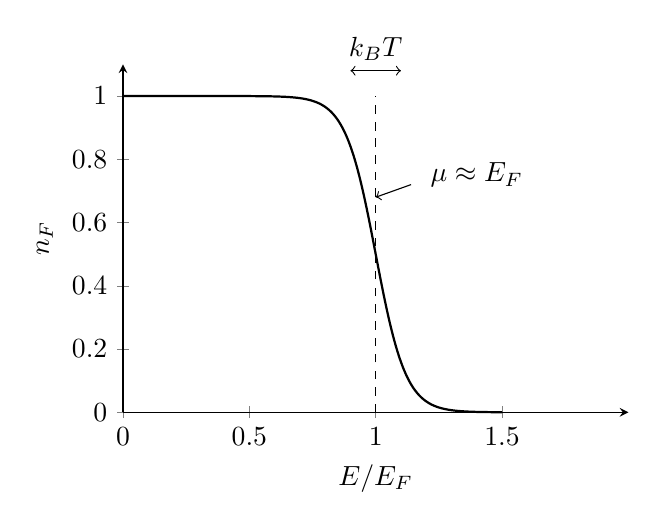
\begin{tikzpicture}
        \begin{axis}[
            width=8cm,
            height=6cm,
            xmin=0, xmax=2,
            ymin=0, ymax=1.1,
            axis lines=left,
            xlabel={$E/E_F$},
            ylabel={$n_F$},
            xtick={0,0.5,1.0,1.5},
            ytick={0,0.2,0.4,0.6,0.8,1.0},
            domain=0:1.5,
            samples=300,
            smooth,
            enlargelimits=false,
            clip=false
        ]

        \addplot[thick] {1/(exp((x-1.0)/0.06)+1)};

        % Dashed chemical potential line
        \addplot[dashed] coordinates {(1.0,0) (1.0,1.0)};

        % Annotation for mu ~ E_F
        \node at (axis cs:1.4,0.75) {$\mu \approx E_F$};
        \draw[->] (axis cs:1.14,0.72) -- (axis cs:1.0,0.68);
                % k_B T width arrow
        \draw[<->] (axis cs:0.9,1.08) -- (axis cs:1.1,1.08);
        \node at (axis cs:1.0,1.15) {$k_B T$};

        \end{axis}
    \end{tikzpicture}
    \caption{Phân bố Fermi khi $k_BT \ll E_F$ Đường nét đứt biểu thị thế hóa học $\mu$ giá trị này xấp xỉ bằng $E_F$. Khi $T=0$ phân bố là một hàm bậc thang, nhưng với $T$ hữu hạn, nó bị trải rộng trên một miền năng lượng có bề rộng vào khoảng $k_BT$.}
    \label{fig:1.4}
\end{figure}
Đầu tiên ta định nghĩa \textbf{Năng lượng Fermi, $E_F$} là giá trị của thế hóa học tại $T=0$, đôi khi người ta sẽ gọi là mức Fermi. Còn những trạng thái được lấp đầy tại thời điểm $T=0$ được gọi là biển Fermi. Thông qua năng lượng Fermi ta có 
thể định nghĩa nhiệt độ Fermi là $T_F = E_F/k_B$ khi đó ta có được vector sóng Fermi là
    \eq{1.50}{E_F = \frac{\hbar^2k^2_F}{2m}.}
Ta xét các electron bị nhốt trong một cái hộp với thể tích là $V= L^3$ thỏa điều kiện biên tuần hoàn
khi đó ta sẽ có được vector sóng và năng lượng được cho như sau
    \eqs{\mathbf{k} = \frac{2\pi}{L}(n_x, n_y, n_z); \quad E = \frac{\hbar^2k^2}{2m}.}
Khi đó ta có tổng số electron được tính bởi
    \eq{1.51}{N = 2\sum_{\mathbf{k}}n_F(\mathbf{k}),}
Ở đây số 2 biểu thị cho mỗi vector sóng có 2 trạng thái spin khả dĩ tuân theo nguyên tắc loại trừ Pauli. Khi áp dụng điều kiện biên tuần hoàn thì ta được
    \eq{1.52}{N = 2\frac{V}{(2\pi)^3}\int d\mathbf{k}n_F(\mathbf{k}).}
Tại $T=0$ thì ta có được $n_F(\mathbf{k}) = 1$ khi đó sẽ rất dễ dàng khi lấy tích phân biểu thức~\eqref{eq:1.52} và chuyển $d\mathbf{k}$ sang hệ tọa độ cầu.
    \eq{1.53}{N = 2\frac{V}{(2\pi)^3}\int_{|\mathbf{k}| < k_F} d\mathbf{k} =  2\frac{V}{(2\pi)^3}\frac{4}{3}\pi k_F^3.}
Với việc mật độ hạt được định nghĩa là $n = N/V = k_F^3 / 3\pi^2$ ta sẽ suy ra được số sóng Fermi là $k_F = (3\pi^2n)^{1/3}$, từ đó ta có năng lượng Fermi là
    \eq{1.54}{E_F = \frac{\hbar^2}{2m}(3\pi^2n)^{1/3} = \frac{1}{2}mv_F^2.}
Nếu ta biết được số electron tự do có trong kim loại thì ta có thể ước tính được năng lượng Fermi, ví dụ đối với đồng (Cu) ta ước lượng được năng lượng khoảng $7eV$ thì ta thu được nhiệt độ Fermi khoảng $8\times 10^4 K$. Tương tự ta cũng 
có thể tính được vận tốc Fermi với giá trị khoảng $1\%c$ đối với Cu.
\subsection{Electronic Heat Capacity}
Nhiệt dung của kim loại sẽ tuân theo biểu thức
    \eq{1.55}{C_v = \alpha T^3 + \gamma T.}
Tương tự với \eqref{eq:1.52} ta có tổng năng lượng của hệ được cho bởi
    \eq{1.56}{E_{\text{tot}} = 2\sum_{\mathbf{k}}\frac{\hbar^2 k^2}{2m}n_F(\mathbf{k}) =  2\frac{V}{(2\pi)^3}\int d\mathbf{k}\frac{\hbar^2 k^2}{2m}n_F(\mathbf{k}).}
Ban đầu như đã nói ta chọn thế hóa học $\mu$ sao cho tổng số hạt trung bình sẽ đúng bằng $N$, thông qua đó một cách gián tiếp nếu ta tìm được số hạt $N$ thì ta sẽ suy ra được thế hóa học $\mu$. Bắt đầu với
    \eq{1.57}{N = 2\frac{V}{(2\pi)^3}\int d\mathbf{k}n_F(\mathbf{k}) = 2\frac{V}{(2\pi)^3}4\pi \int_0^{\infty} dk k^2 n_F(\mathbf{k}).}
Khi này ta đặt $k = \sqrt{2Em/\hbar^2}$ khi đó tích phân trên được viết lại là
    \eq{1.58}{N = 2\frac{V}{(2\pi)^3}4\pi\int_0^{\infty} dE n_F \frac{m}{\hbar^2}\sqrt{\frac{2mE}{\hbar^2}} = V  \int_0^{\infty} dE n_F \frac{1}{2\pi^2}\left(\frac{2m}{\hbar^2}\right)^{3/2}E^{1/2}.}
Khi đó ta đặt
    \eq{1.59}{g(E) = \frac{1}{2\pi^2}\left(\frac{2m}{\hbar^2}\right)^{3/2}E^{1/2}.}
Được gọi là mật độ trạng thái trên một đơn vị thể tích. Với $g(E)dE$ chính là tổng số trạng thái riêng (eigenstates) bao gồm cả hai trạng thái spin có năng lượng nằm trong khoảng từ $E \rightarrow E + dE$. Khi $T = 0$ hàm Fermi là một hàm bậc thang và thế hóa học chính là năng lượng Fermi, đối với nhiệt độ $T$ nhỏ thì hàm bậc thang bị trải rộng trên một miền năng lượng có bề rộng vào khoảng $k_BT$ như hình~\ref{fig:1.4}.
Và điều đặc biệt ta có thể thấy được đó là số lượng các trạng thái bị loại bỏ từ bên dưới mức thế hóa học gần như hoàn toàn bằng với số lượng các trạng thái được thêm vào phía trên mức thế hóa học, do đó ta có thể kết luận $\mu \approx E_F$ đối với bất kỳ nhiệt độ thấp nào. Nhưng chi tiết hơn thì thế hóa học có dạng chính xác hơn là
    \eq{1.60}{\mu = E_F + \mathcal{O}(T/T_F)^2.\footnote{Xem chương 2 sách Ashcroft, Mermin, \textit{Solid State Physics}.}}
Thông qua hình~\ref{fig:1.4} ta có thể thấy rằng chỉ những electron nằm trong dải năng lượng cỡ $k_BT$ xung quanh mặt Fermi mới có thể bị kích thích và chúng bị kích thích lên trên mặt Fermi đúng bằng một khoảng năng lượng $k_BT$. Khi đó ta có phép xấp xỉ
    \eqs{E(T) = E(T=0) + (\text{number of electrons excited}) \times (\text{energy absorbed})}
Khi đó biểu diễn ta ta được
    \eq{1.61}{E(T) = E(T=0) + \frac{\tilde{\gamma}}{2}(Vg(E_F)k_BT)\times(k_BT),}
Trong đó $\tilde{\gamma} = \pi^2/3$. Khi đó ta tính được nhiệt dung
    \eq{1.62}{C = \frac{\partial E}{\partial T} = \tilde{\gamma}\left(\frac{3}{2}k_BT\right)\left(\frac{T}{T_F}\right).\footnote{Biến đổi dựa trên biểu thức~\eqref{eq:1.59} và \eqref{eq:1.61}.}}
Ta có thể nhận ra rằng là nhiệt dung của khí electron sẽ bé hơn rất nhiều so với nhiệt dung của khí cổ điển do hệ số $T/T_F \lesssim 0,01$. Ta đã thấy ở phương trình~\eqref{eq:1.48} Drude dự đoán hệ số Seebeck chênh lệch cỡ 100 lần, nguyên nhân của sai số này là do trong phép tính đó 
ta đã sử dụng nhiệt dung tính trên mỗi electron của một hệ khí cổ điển, giá trị này lớn hơn thực tế khoảng $T_F/T \approx 100$.
Ta cũng đã sử dụng nhiệt dung trên mỗi hạt trong phép tính của Drude về độ dẫn nhiệt, giá trị của $\langle v \rangle$ mà ông dùng lại quá nhỏ với một hệ số gần như tương đương (trong bức tranh cổ điển, người ta sử dụng $mv^2/2 \thicksim k_BT$ trong khi đối với mô hình Sommerfeld, ta phải sử dụng vận tốc Fermi
$mv^2_F \thicksim k_BT_F$), nhờ sự bù trừ này, dự đoán của Drude về độ dẫn nhiệt lại cho ra kết quả xấp xỉ đúng (và nhờ vậy định luật Wiedemann - Franz vẫn hoàn toàn chính xác).
\subsection{Magnetic Spin Susceptibility (Pauli Paramagnetism)}
Trong cơ lượng tử ta biết nếu một hạt di chuyển với quỹ đạo tròn (tức đang quay) thì nó sẽ tạo thành một moment lưỡng cực từ, khi đó moment lưỡng cực của nó là $\mathbf{\mu}$ sẽ tỉ lệ với moment động lượng spin $\mathbf{S}$
    \eq{1.63}{\mathbf{\mu} = \gamma \mathbf{S}.}
Trong đó $\gamma$ là tỉ số hồi chuyển từ (gyromagnetic ratio). Nếu ta đặt một lưỡng cực từ vào trong một từ trường $\mathbf{B}$ thì nó sẽ chịu một moment lực $\mathbf{\mu}\times\mathbf{B}$, moment xoắn này có xu hướng làm cho nó song song với từ trường, khi đó năng lượng của moment xoắn này là
    \eq{1.64}{U = -\mathbf{\mu}\cdot\mathbf{B} = -\gamma \mathbf{S}\cdot\mathbf{B}}
Trong đó $\gamma <0$ đối với electron và được tính là $\gamma = -e/m$, và ta cũng biết ta có chuyển $\mathbf{S}$ về các ma trận Pauli với trị riêng là $\hbar/2$. Khi đó ta có thể viết lại \eqref{eq:1.64} là
    \eq{1.65}{U = \frac{e\hbar}{2m}\mathbf{\sigma}\cdot\mathbf{B}=\mu_B\mathbf{\sigma}\cdot\mathbf{B}.}
Trong đó $\mu_B$ là Bohr magneton. Khi đó ta có Hamiltonian khi bỏ qua lực Lorentz của từ trường được cho bởi
    \eq{1.66}{\mathscr{H}=\frac{\mathbf{p}^2}{2m}+g\mu_B\mathbf{\sigma}\cdot\mathbf{B}.}
Trong đó $g$ là hệ số $"g"$ của electron và để không bị nhầm lẫn với mật độ trạng thái thì theo sách của Simon ta sẽ đặt $g=2$, và $\mathbf{\sigma}$ là ma trận Pauli và có trị riêng là $\pm 1/2$, thế tất cả vào \eqref{eq:1.66} ta được
    \eq{1.67}{\mathscr{H}=\frac{\mathbf{p}^2}{2m}\pm \mu_B\mathbf{B}.}
Do đó năng lượng của một electron với spin up và spin down đặt trong từ trường được cho bởi
    \eqs{
        \begin{cases}
            \epsilon(\mathbf{k}, \uparrow) &= \dfrac{\hbar^2 |\mathbf{k}|^2}{2m} + \mu_B B \\[10pt]
            \epsilon(\mathbf{k}, \downarrow) &= \dfrac{\hbar^2 |\mathbf{k}|^2}{2m} - \mu_B B.
        \end{cases}
    }
\indent Ta có độ từ hóa (magnetization) được định nghĩa là tổng moment lưỡng cực từ trên một đơn vị thể tích
    \eq{1.68}{M = \frac{\sum\mu}{V} = n_{\uparrow}\mu_{\uparrow} + n_{\downarrow}\mu_{\downarrow}.}
Trong đó ta biến đổi $\mu_{uparrow} = -e\hbar/2m = - \mu_B$, ta có thể viết lại 
    \eq{1.69}{M =  n_{\uparrow}(-\mu_B) + n_{\downarrow}(\mu_B) = \mu_B( n_{\downarrow} - n_{\uparrow}).}
Khi ta đặt electron vào từ trường thì năng lượng của electron bị dịch chuyển do hiệu ứng Zeeman, tức là electron spin up bị tăng một khoảng năng lượng $\mu_B B$ trong khi đó electron spin down lại giảm đi một khoảng năng lượng $\mu_B B$ được mô tả trong hình \ref{fig:1.5}
    \fig{figure/chap1/3.png}{0.6}{Khi không có từ trường thì mật độ trạng thái của spin up và spin down là như nhau, $g_{\uparrow}(E)=g_{\downarrow}(E)=g(E)/2$. Khi đặt trong từ trường thì do hiệu ứng Zeeman mà năng lượng dịch chuyển một khoảng $\pm \mu_B B$}{1.5}
\noindent Khi đó ta tính được mật độ số hạt là
    \eqs{n_{\uparrow} = \frac{N_{\uparrow}}{V} = \int_{0}^{E_F - \mu_B B} \frac{g(E)}{2} dE}
    \eqs{n_{\downarrow} = \frac{N_{\downarrow}}{V} = \int_{0}^{E_F + \mu_B B} \frac{g(E)}{2} dE}
Từ đó suy ra
    \eq{1.70}{n_{\downarrow} - n_{\uparrow} = \int_{E_F - \mu_B B}^{E_F + \mu_B B} \frac{g(E)}{2} dE = \frac{g(E_F)}{2}2\mu_B B.}
Thế \eqref{eq:1.70} vào \eqref{eq:1.69} ta được
    \eq{1.71}{M = g(E_F)\mu_B^2 B = \chi B.}
Trong đó $\chi = g(E_F)\mu_B^2$ gọi là magnetic susceptibility. Ta có
    \begin{enumerate}
        \item $\chi > 0$: thuận từ (Paramagnetism).
        \item $\chi < 0$: nghịch từ (Diamagnetism).
        \item $M \neq 0$ kể cả khi $B = 0$: sắt từ (Ferromagnetism).
    \end{enumerate}
Những phần còn lại như là tại sao lý thuyết Drude hoạt động tốt hay những hạn chế của mô hình electron tự do thì mời các bạn đọc thêm trong sách của Steven H. Simon, \textit{The Oxford Solid State Basics}.
\let\cleardoublepage\clearpage
